\documentclass[a4paper,11pt]{report}
\usepackage[utf8]{inputenc}
\usepackage{color,amsmath,xcolor,listings,graphicx}
\usepackage[francais]{babel}

%% infos du document
%%\title{Bureau d'étude 2014 - Télécommunication : Courant Porteur de Lignes \\\& \\Filtres}
\title{Courant Porteur de Lignes \\ \& \\Filtres}
\author{Loïc Barbaresco, Rémi Barbaste, Robin Degironde, Émeric Tosi}
\date{\today}


\begin{document}

%% Afficher la page de garde : Titre + Auteur(s) + Date de dernière compilation
    \maketitle{}


%    \begin{figure}
%        \begin{center}
            %%% au choix
            %\includegraphics{image.png}
            %\includegraphics[height=128, width=128]{image.png}
            %\includegraphics[scale=0.5]{image.png}
%        \end{center}
%            \caption{ Laule } % ce qui apparait juste en dessous de l'image
%            \label{c'est styler !}
%    \end{figure}

    \setcounter{tocdepth}{1} % définir la profondeur de l'Index
    \renewcommand{\contentsname}{Sommaire} % renommer l'Index en Sommaire
    \tableofcontents{} % afficher l'Index
    \clearpage


%% Partie principale :
    
\part*{Introduction}
    \paragraph{}
Dans le cadre de notre formation Système Télécommunication et Réseaux Informatiques, nous avons réalisé un bureau d'étude.
Le but de ce bureau d'étude est l'analyse d'un problème, l'écriture de sa problématique associée,
l'organisation des différentes tâches, ainsi que la synthèse du travail réalisé sur cette problématique.
Nous nous sommes aussi préparés à répondre à des questions d'un public sur notre thème de recherche.
    \paragraph{}
Notre thème porte sur : « Les courants porteurs de ligne ».
    \paragraph{}
De nos jours de plus en plus de maisons sont équipées d'objets et d'automatismes connectés, on parle alors de domotique et de maison connectée.
Cette représente le croisement entre les fruits des recherche en électronique, en automatisme, en médecine, en ergonomie et en génie civil.
La domotique a pour but de faciliter et d'automatiser les tâches du quotidien et actions nécessaires ou utiles dans un bâtiment,
ici une maison individuelle, par le biais de réseaux locaux entres appareils.
    \paragraph{}
Cette technologie utilise un certain nombre d'appareils pouvant être vu comme des terminaux distributeurs de données et/ou actionneurs.
Il est nécessaire de les interconnecter afin qu'ils puissent d'une part échanger entre eux,
et d'autre part avec une console interface homme-machine par exemple.
    \paragraph{}
Suivant le type de construction, sa vétusté et sa disposition, la mise en place d'un tel système peut s'avérer très complexe.
De multiples solutions existent dont la technologie du courant porteur de ligne.

\addcontentsline{toc}{part}{Introduction}
    \clearpage


\part*{Problématique}
    \section*{En quoi les CPL peuvent-ils faciliter le développement des objets connectés dans les maisons individuelles ?}
\addcontentsline{toc}{part}{Problématique}
    \clearpage


%%%%
\part{La Domotique et les objets connectés}
    \section{La Domotique}
        \paragraph{}
La domotique est le croisement entre l’ensemble des techniques de l’électronique, informatique, automatisme et bâtiment.
        \paragraph{}
Son but est d’automatiser et de centraliser tous les appareils présents dans une maison
(du volet roulant en passant par le système de chauffage ou les éclairages) afin d'assurer :
            \begin{itemize}
                \item le confort optimal (portails automatiques, stores électriques, chauffages régulés);
                \item la sécurité des biens et personnes.
            \end{itemize}
        \paragraph{}
De nos jours de différentes thématiques apparaissent :
            \begin{itemize}
                \item la gestion des énergies autant économique qu'éco-responsable;
                \item l'assistance aux handicapés.
            \end{itemize}
        \begin{figure}[h]
            \begin{center}
                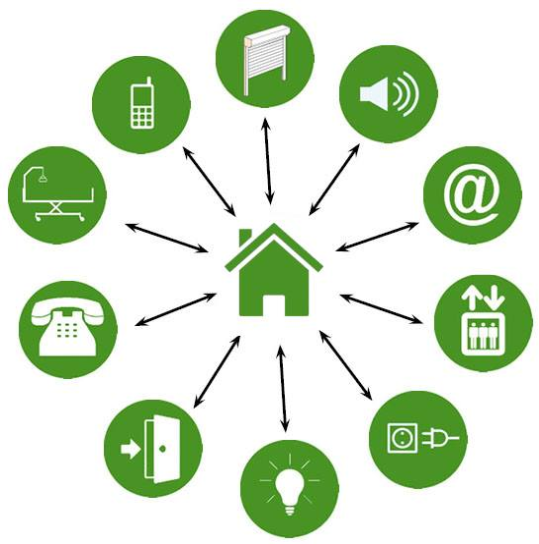
\includegraphics[scale=0.4]{./images/cpl/partieDomotique.png}
            \end{center}
                \caption{ Usages de la domotique } % ce qui apparait juste en dessous de l'image
                \label{Usages de la domotique}
        \end{figure}
        \paragraph{}
De nos jours les utilisateurs exigent d'avantage de commandes à distance de tous leurs équipements sans que ces derniers perdent en autonomie ou en facilité d'utilisation.
Nous entrons dans l’ère de la domotique commandée à distance, qui se ne se contente plus d'automatiser les services :
comment commander son installation avec son terminal depuis n'importe ou ?
        \paragraph{}
C’est ce que l’on appelle l’internet des objets.
Très en vogue de nos jours, en particulier dans le domaine de l’électroménager (frigo, cafetière ...)
dans le but d'un déclenchement automatique ou d'alarme d'état de l'équipement, toujours dans l’optique d’un meilleur confort.
        \paragraph{}
Le système domotique étant mis en réseau (et souvent connecté à internet), il est désormais possible de le piloter de n’importe où.
Une personne peut très bien ouvrir les volets ou la porte de son garage sur son smartphone en étant au bureau.
La programmation de ces actions est aussi possible et les différents appareils communiquent entre eux afin de connaître leur état.
        \paragraph{}
Même si certains protocoles logiciels sont propriétaires, les appareils se doivent de pouvoir communiquer sur un réseau informatique grand public,
puisqu’ils seront pilotés par des applications sur des terminaux conventionnels tels que des ordinateurs ou des smartphones.
On utilise donc des standards de l’informatique pour l’interconnexion des appareils :
            \begin{itemize}
                \item Câble Réseau;
                \item WIFI;
                \item RF433;
                \item CPL.
            \end{itemize}
        \paragraph{}
Dans ce BE nous avons choisi de nous orienter sur le CPL qui nous parait être une solution plus pérenne.


    \clearpage
    \section{CPL, Courant Porteur de Ligne}
        \subsection{Principes de cette technologie}
            \paragraph{}
La technologie du courant porteur en ligne (CPL) sert à transporter un signal haute fréquence de 1.6 à 30 MHz en le superposant au signal 50Hz du courant électrique du secteur.
Il est ainsi possible de créer un réseau local avec accès Internet haut débit avec le réseau électrique d'un logement.
Les câbles électriques déjà présents dans les habitations permettent donc la mise en réseau d'ordinateurs et de matériels.
    \begin{figure}[h]
        \begin{center}
            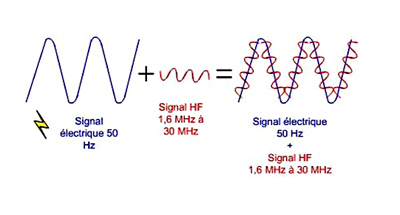
\includegraphics[scale=0.7]{./images/cpl/principeCpl.jpg}
        \end{center}
            \caption{ Schéma du principe du CPL } % ce qui apparait juste en dessous de l'image
            \label{Principe du CPL}
    \end{figure}

        \subsection{Fonctionnement et technique}
            \paragraph{}
La signal de la transmission des données est atténuée par différents critères comme l’ancienneté et l'état du réseau électrique, la longueur des câbles, l'utilisation de multi-prises, la présence d'autres appareils perturbant le signal ou encore la qualité des adaptateurs CPL utilisés.
Le CPL est une alternative très intéressante aux long câbles Ethernet et au Wi-Fi à la sécurité et à la pollution électro-magnétique controversées.
Créer son réseau local et partager sa connexion haut débit devient alors aussi simple que de brancher n'importe quel appareil sur une prise électrique murale.

    \begin{figure}[h]
        \begin{center}
            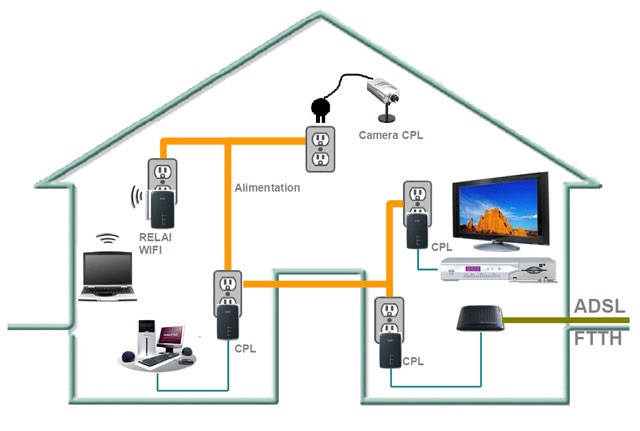
\includegraphics[scale=0.5]{./images/cpl/exempleReseauLocalCPL.jpg}
        \end{center}
            \caption{ Exemple de réseau local par CPL avec accès Internet haut débit } % ce qui apparait juste en dessous de l'image
            \label{Exemple liens actuels avec CPL}
    \end{figure}

        \subsection{Normes et hétérogénéité}
            \paragraph{}
Avant d’en dire plus sur les débits observés dans les réseaux CPL, il est important de faire la différence entre deux types de réseaux,
les réseaux «indoor» et «outdoor».
            \paragraph{Les réseaux «indoor» (intérieur)}
,il s'agit de câbles électriques situés entre le compteur électrique et tous les équipements d’un logement.
Il est ainsi possible d'avoir un réseau composé uniquement d'une structure utilisant les réseaux CPL.
Il est aussi possible d'associer au réseau CPL, des équipements Ethernet (tels que des switch, des routeurs, des modems, des bornes d'accès wifi...)
tout en ne dépassant pas les limitations concernant le nombre d'utilisateurs ou de matériels connectés sur ces réseaux locaux.
            \paragraph{Les réseaux «outdoor» (extérieur)}
,il s'agit des câbles situés entre le compteur électrique et le transformateur général du quartier.
On parle souvent de mise en place d’une boucle locale ou “dernier kilomètre”.
Cette boucle relie les différentes habitations ou lieux où l'on veut mettre en place une solution CPL.
Cette partie est gérée par le fournisseur d'accès.
            \paragraph{}
Du fait de ce découpage, un certain nombre de matériels vont être nécessaires pour relier les lieux en extérieur et les matériels en intérieur.
Il n'est pas possible d'utiliser l'ensemble du réseau électrique pour fournir un accès à des réseaux plus globaux tels que l’internet.
Le point d'entrée global, à savoir le transformateur ou la station électrique de quartier ne peut être réaliser en CPL car il s'agit d'une partie haute tension.
Les réseaux CPL ne peuvent fonctionner que sur de basses et moyennes tensions, pour des problèmes d'interférences et de bruit électromagnétique.
            \paragraph{}
Voici quelques exemples des débits disponible actuellement sur le marché :
                \begin{itemize}
                    \item 14 Mbits/s \emph{(dépassé)} ;
                    \item 85 Mbits/s \emph{(dépassé)} ;
                    \item 200 Mbits/s \emph{(le strict minimum)} ;
                    \item 500 Mbits/s ;
                    \item 600 Mbits/s ;
                    \item 650 Mbits/s \emph{range+ chez Devolo} ;
                    \item 1 Gbit/s (1000 Mbits/s) \emph{avec prises de terre uniquement}.
                \end{itemize}
            \paragraph{}
Tout comme pour les débits WiFi, 7 Gbits/s théorique pour le 802.11ac sur 8 bandes,
les débits annoncés et réel pour le courant porteur en ligne ne sont pas égaux.
Les vitesses réellement observées varient globalement de 45 à 75\% par rapport aux débits annoncés.
Pour un adaptateur CPL 600 Mbits/s, cela permet tout de même des débits moyens tournant autour des 450 Mbits/s, soit près de 60 Moctets/s.


    \clearpage

%%%%
\part{Produits actuellement disponibles}
    \paragraph{}
Pourquoi avons vous choisi de mettre en avant le CPL dans la domotique plutôt que la WIFI ou le câble réseau classique ?
    \paragraph{}
Le choix de la technologie du support de communication se repose sur trois points essentiels :
        \begin{itemize}
            \item La sécurité;
            \item Le coût;
            \item La topologie du bâtiment.
        \end{itemize}
    \paragraph{}
En effet, selon l’utilisation, le critère de sécurité est mis en avant.
Comparons avec une interconnexion basé sur des réseaux WIFI : l’espace ambiant est le support des communications.
L’avantage indéniable est sa mise en place rapide et peu coûteuse.
L’inconvénient est que cet espace est accessible à tous, certes il y a des protections d'accès au réseau (WEP, WPA/WPA2)
mais il existe des méthodes d’attaque de plus en plus rapides et simples pour s’introduire dans le réseau utilisé par l’appareillage domotique.
De plus, pour une installation la surface n'est pas négligeable et les murs sont susceptible de filtrer le signal (béton armé, armature zinc-placo).
Il serait indispensable d’installer des répéteurs WIFI afin d’étendre le signal, tout cela invalide l’argument du «peu coûteux».

        \begin{figure}[h]
            \begin{center}
                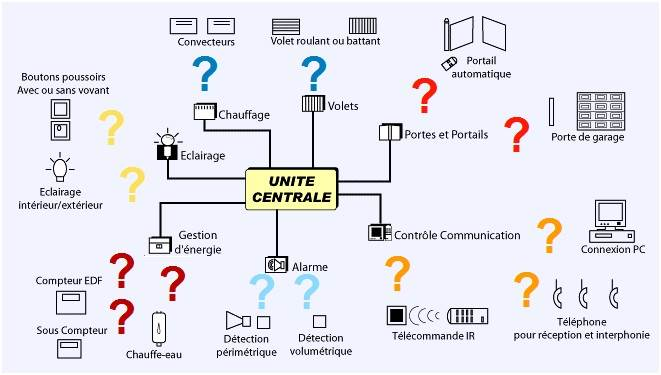
\includegraphics[scale=0.4]{./images/cpl/imageUniteCentrale.jpg}
            \end{center}
                \caption{ Exemple de domotique à la structure de réseau dépassée } % ce qui apparait juste en dessous de l'image
                \label{Exemple de domotique avec commande centrale}
        \end{figure}

    \paragraph{}
La topologie de type filaire est la meilleure du point de vue sécurité, car pour s'introduire sur le réseau la seule possibilité est d’accéder au support physique.
Pour une installation de ce type il faut cependant dépenser un budget considérable dans l’achat de longueurs de câble et d'équipements d’interconnexion.
De plus, pour un bâtiment existant et non équipé, il faut compter en plus le passage des câbles et la modification de la structure entraînant un nouvel investissement financier.
    \paragraph{}
Les bâtiments existants sont donc particulièrement difficiles à équiper et c’est là que la technologie CPL prends tout son sens.
Le support physique utilisé est l’installation électrique existante.
Un bâtiment classique possède déjà une installation électrique, ce qui signifie qu'il n'y a pas d’investissements à faire dans le déploiement du support de communication.
Il n’y a pas non plus d’équipement d’interconnexion à nécessairement utiliser ce qui est un avantage du point de vue budgétaire.
La portée point à point d’un équipement CPL peut aller jusqu’à 300m.
Étant donné que le support utilisé est aussi filaire, le seul moyen de s’introduire sur le réseau électrique du logement.
Cela est moins sûr que Ethernet mais réduit grandement les risques d’intrusion par rapport à la WIFI.

        \begin{figure}[h]
            \begin{center}
                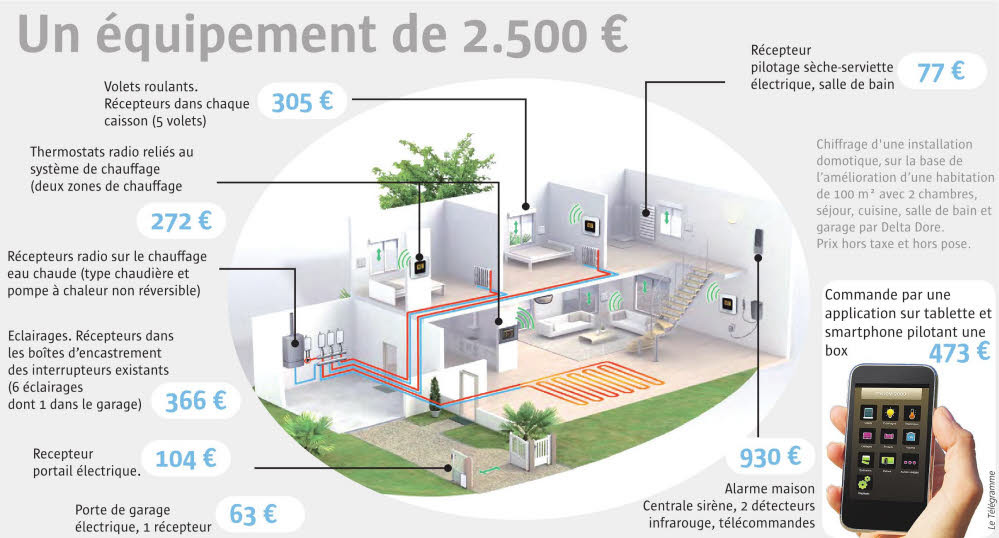
\includegraphics[scale=1.5]{./images/cpl/exempleMaisonIntelligente.jpg}
            \end{center}
                \caption{ Exemple de maison intelligente disponible } % ce qui apparait juste en dessous de l'image
                \label{Exemple de maison intelligente disponible}
        \end{figure}


    \clearpage
%%%%
\part{Exemple type}
            \paragraph{}
Cette partie va être consacrée à une étude d’un exemple que l’on peut trouver dans une maison individuelle.
Il va nous permettre de vous montrer que les CPL peuvent être très utilisés dans la domotique.
            \paragraph{}
Dans cette maison, on rencontre des équipements intelligents pour le chauffage, la production d’eau chaude, l’éclairage et la sécurité.
Grâce à ces équipements, nous pouvons gérer la température dans différentes pièces pour le chauffage par exemple, ou l'humidités pour la ventilation dans une salle de bain après une douche.
Tous ces appareils peuvent être inter-connectés grâce à des CPL qui peuvent transmettre les informations instantanément au compteur électrique, pour éviter les pics de consommation énergétique.
Ainsi nous pourrons réduire les factures en étalant le fonctionnement de l'électroménager.
Nous pouvons aussi étendre ce système à l’éclairage de la maison avec des détecteurs de mouvement qui peuvent allumer une lumière à l’arrivée d’une personne,
des détecteurs de luminosité pour ouvrir les volets le jour, ou même allumer les différentes pièces pour simuler une présence et ainsi prévenir les cambriolages.
Cela permet d'interagir avec les équipements une fois parti de la maison à notre guise, sur notre smartphone, tablette, ou autre terminal.
Les risques d’incendie sont réduits en désactivant, par prise en main à distance ou automatiquement, des appareils puissants oubliés.
            \paragraph{}


%%%
%%%
%%%
%%%
%%%
%%%
%%%
%%%
%%%
%%%
%~ \part{AUTRES}
        %~ \section{Qu’est-ce que c’est ?}
%~ La domotique est l’ensemble des techniques de l'électronique, de physique du bâtiment, d'automatisme, de l'informatique et des télécommunications utilisées dans les bâtiments, plus ou moins « interopérables » et permettant de centraliser le contrôle des différents systèmes et sous-systèmes de la maison et de l'entreprise (chauffage, volets roulants, porte de garage, portail d'entrée, prises électriques, etc.).
%~ La domotique vise à apporter des solutions techniques pour répondre aux besoins de confort (gestion d'énergie, optimisation de l'éclairage et du chauffage), de sécurité (alarme) et de communication (commandes à distance, signaux visuels ou sonores, etc.) que l'on peut retrouver dans les maisons, les hôtels, les lieux publics, etc.
            %~ \paragraph{}
%~ le pilotage des appareils « électro-domestiques », électroménagers par programmation d'horaires et/ou de macro (suites d'actions programmées réalisées par les appareils électroménagers) définis par l'usager. Le déclenchement des appareils peut être aussi lié à des évènements (détecteurs de mouvement, télécommandes, etc.) ;
%~ la gestion de l'énergie, du chauffage (par exemple, il est possible de gérer les apports naturels (calories, frigories, vent, lumière, eau…) en fonction de l'enveloppe thermique du bâtiment), de la climatisation, de la ventilation, de l'éclairage, de l’ouverture et de la fermeture des volets (en fonction de l'ensoleillement ou de l'heure de la journée, par exemple), de l'eau (le remplissage de la baignoire peut s’arrêter automatiquement grâce à un senseur, les robinets de lavabos peuvent ouvrir l’eau à l’approche des mains, etc.). Il est également possible de recharger certains appareils électriques (ordinateurs, véhicules électriques, etc.) en fonction du tarif horaire (voir Smart grid). Un compteur communicant peut être intégré dans un smart-grid et/ou raccordé à un système de télégestion. La Régulation/programmation du chauffage permet d'importantes économies ;
%~ la sécurité des biens et des personnes (alarmes, détecteur de mouvement, interphone, digicode) ;
%~ la communication entre appareil et utilisateur par le biais de la « son-ification » (émission de signaux sous forme sonore) ;
%~ le « confort acoustique ». Il peut provenir de l'installation d'un ensemble de haut-parleurs permettant de répartir le son et de réguler l’intensité sonore ;
%~ la compensation des situations de handicap et de dépendance.
%~ Elle peut aussi chercher à diminuer son empreinte écologique (« éco-domotique ») et celle de ses utilisateurs par une éco conception, en facilitant une meilleure maîtrise de la consommation énergétique de l'habitat, en améliorant l'efficience énergétique des installations
            %~ \paragraph{}
%~ Avec le temps, la domotique tend à sortir de la maison. Elle met par exemple en relation des unités d'habitation entre elles et avec un immeuble (c'est l'immotique) et avec la ville (on entre alors dans l'« urbatique » et/ou avec un gestionnaire / propriétaire et/ou d'autres entités fournissant par exemple des services (eau, énergie, livraison de nourriture, soins à domicile ou distant, lavage de vêtements, etc). Si ces services visent prioritairement à moins dégrader l'environnement, on parle parfois d'« éco domotique urbaine ».
            %~ \paragraph{}
%~ Ces coûts proviennent essentiellement pour 60 \% de la partie électrique (main d’œuvre électricien, nombres d’éléments à contrôler, nombre de capteurs, nombre de pièces, etc.) et pour environ 40 % de la partie chauffage (nombre de pièces à chauffer, nombre de radiateurs, etc.). Par ailleurs, le coût d'évolution est plus élevé, des travaux importants pouvant être nécessaire pour compléter le réseau.
            %~ \paragraph{Exemples de scénarios :}
            %~ %    \begin{figure}
            %~ %        \begin{center}
                        %~ %%% au choix
                        %~ %\includegraphics{image.png}
                        %~ %\includegraphics[height=128, width=128]{image.png}
                        %~ %\includegraphics[scale=0.5]{image.png}
            %~ %        \end{center}
            %~ %            \caption{ Laule } % ce qui apparait juste en dessous de l'image
            %~ %            \label{c'est styler !}
            %~ %    \end{figure}
%~ en partant au travail, un simple clic sur un interrupteur installé dans l’entrée enclenche le scénario « départ au travail ».
%~ L’éclairage s’éteint, le garage s’ouvre, le chauffage se met en veille au bout de 15 minutes, les volets et le garage se ferment après 30 minutes ;
%~ en quittant le travail pour rentrer chez soi, on actionne le scénario de retour à l’aide du téléphone WAP ou depuis l’ordinateur du bureau : les volets s’ouvrent et le chauffage passe en mode confort ;
%~ quand on est fatigué, on agit sur la télécommande de la maison afin d’enclencher le scénario « relaxation », les lumières se tamisent, un fond sonore apaisant se propage dans la pièce.
%~
%~
    %~ \section{CPL}
        %~ \subsection{Définition du CPL}
            %~ \paragraph{Courant porteur ligne}
%~ La transmission des données est atténuée par différents critères comme la vétusté du réseau électrique, la longueur des câbles, l'utilisation de multiprises, la présence d'autres appareils perturbant le signal ou encore la qualité des adaptateurs CPL utilisés.
%~ Néanmoins, le CPL est une alternative très intéressante aux câbles disgracieux et au Wi-Fi pas toujours très sécurisé.
%~ Créer son réseau local et partager sa connexion haut-débit devient alors aussi simple que de brancher n'importe quel appareil sur une prise électrique murale.
            %~ \paragraph{Principes de cette technologie}
%~ La technologie du courant porteur en ligne (CPL) permet de transporter un signal de haute fréquence en le superposant au signal 50hz du courant électrique qui est délivré par les traditionnelles prises de courant.
%~ Grâce à la transmission d'informations numériques sur le réseau électrique 220 Volts existant, il est ainsi possible de créer un réseau local Internet haut-débit avec le réseau électrique d'un logement.
%~ S'appuyant sur les câbles électriques déjà présents dans la plupart des habitations, le CPL permet la mise en réseau d'ordinateurs et de matériels équipés d'une prise RJ45 (Ethernet), dans un appartement, un bureau ou une maison, avec un débit théorique de transfert des données de l'ordre de plusieurs centaines de mégabits par seconde.
    %~ \section{Etude de l’art}
            %~ \paragraph{Normes et hétérogénéité}
%~ Tout comme pour les débits WiFi, \emph{ le \emph{802.11n} étant limité pour l'instant à 300 Mbits/s, le \emph{802.11ac} en double-bande aux alentours de 1900 Mbits/s}, les débits annoncés (\emph{théoriques}) pour le courant porteur en ligne ne sont pas aussi importants dans la réalité.
%~ Ainsi, les vitesses réellement observées varient globalement de 45 à 75\% par rapport aux débits annoncés.
%~ Pour un adaptateur CPL 600 Mbits/s, cela permet tout de même des débits moyens tournant autour des 450 Mbits/s, soit près de 60 Mio/s.


    \clearpage

%% Annexes
    
\part*{Annexes}
    \paragraph{}
lolilol !


\addcontentsline{toc}{part}{Annexes}

    \clearpage

%% Index des images du rapport
    \listoffigures
    \clearpage

\end{document}
